% f2015hnw_q18_prism.tex — 2015 年高考数学·湖南卷·文科 第 18 题（三棱柱）
%
% 【来源】`.work/phase3-b22/source/2015湖南文.pdf`（SHA-256
%   48dc0c6771ccea8291a3ac94336dd89a8b4ff89fa6baceaa76585c349582a074），
%   第 2 页（合订本页 958）；内容对象 21。逐路径实测见
%   `.work/phase3-b22/figure-inventory.md`。
%
% 【坐标口径】源 PDF 用户空间（原点左下、y 向上）。本图本地坐标
%   (x, y) = (x_page − 279.71, y_page − 586.523)，1 单位 = 1 TeX pt。
%   路径坐标逐点照录内容流（含三次贝塞尔控制点）。
%
% 元素计数：13 条路径（9 实＋4 虚）＋8 个标签
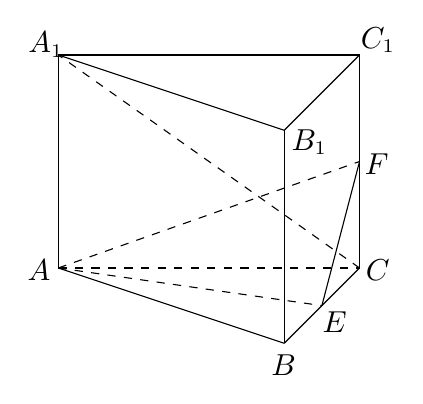
\begin{tikzpicture}[x=1pt, y=1pt,
    every node/.style={inner sep=0pt, font=\fontsize{10.5pt}{12.6pt}\selectfont}]
  \draw[line width=0.3985pt] (81.6302,-0.0002)   (81.6302,-0.0002)   -- (108.8459,27.2070);
  \draw[line width=0.3985pt] (0.0001,27.2070)   (0.0001,27.2070)   -- (81.6302,-0.0002);
  \draw[line width=0.3985pt] (0.0001,27.2070)   (0.0001,27.2070)   -- (0.0001,104.1723);
  \draw[line width=0.3985pt] (81.6302,-0.0002)   (81.6302,-0.0002)   -- (81.6302,76.9650);
  \draw[line width=0.3985pt] (108.8459,27.2070)   (108.8459,27.2070)   -- (108.8459,104.1723);
  \draw[line width=0.3985pt] (0.0001,104.1723)   (0.0001,104.1723)   -- (81.6302,76.9650);
  \draw[line width=0.3985pt] (81.6302,76.9650)   (81.6302,76.9650)   -- (108.8459,104.1723);
  \draw[line width=0.3985pt] (108.8459,104.1723)   (108.8459,104.1723)   -- (0.0001,104.1723);
  \draw[line width=0.3985pt] (95.2381,13.6034)   (95.2381,13.6034)   -- (108.8459,65.6898);
  \draw[line width=0.3985pt, dash pattern=on 2.98883pt off 2.98883pt, dash phase=0.0pt] (0.0001,27.2070)   (0.0001,27.2070)   -- (95.2381,13.6034);
  \draw[line width=0.3985pt, dash pattern=on 2.98883pt off 2.98883pt, dash phase=0.0pt] (0.0001,27.2070)   (0.0001,27.2070)   -- (108.8459,27.2070);
  \draw[line width=0.3985pt, dash pattern=on 2.98883pt off 2.98883pt, dash phase=0.0pt] (0.0001,27.2070)   (0.0001,27.2070)   -- (108.8459,65.6898);
  \draw[line width=0.3985pt, dash pattern=on 2.98883pt off 2.98883pt, dash phase=0.0pt] (108.8459,27.2070)   (108.8459,27.2070)   -- (0.0001,104.1723);

  \node[anchor=center] at (-6.970,26.247) {$A$};  % 源中心 (272.74,612.77)
  \node[anchor=center] at (81.370,-7.933) {$B$};  % 源中心 (361.08,578.59)
  \node[anchor=center] at (115.440,26.247) {$C$};  % 源中心 (395.15,612.77)
  \node[anchor=center] at (-4.510,107.977) {$A_1$};  % 源中心 (275.20,694.50)
  \node[anchor=center] at (90.690,72.677) {$B_1$};  % 源中心 (370.40,659.20)
  \node[anchor=center] at (115.490,109.477) {$C_1$};  % 源中心 (395.20,696.00)
  \node[anchor=center] at (99.870,7.707) {$E$};  % 源中心 (379.58,594.23)
  \node[anchor=center] at (115.090,64.727) {$F$};  % 源中心 (394.80,651.25)

\end{tikzpicture}
%
% 【自验结果】
%   探针：latexmk -pdfxe（待跑）。
